\documentclass{article}
\usepackage[utf8]{inputenc}
\usepackage{amsmath}
\usepackage{amssymb}
\usepackage{graphicx}
\usepackage{tikz}
\usepackage{geometry}
 \geometry{
 a4paper,
 total={210mm,297mm},
 left=10mm,
 top=30mm,
 right=10mm
 }

\graphicspath{{./}}
\newcommand*\circled[1]{\tikz[baseline=(char.base)]{
    \node[shape=circle,draw,inner sep=0.5pt] (char) {#1};}}

\title{ 
\normalfont \large 
\textsc{Indian Institute of Technology, Ropar} \\    [40pt] 
\horrule{} \\[0.4cm] 
\Huge CS204 Course Project - Phase I\\ 
\horrule{} \\[0.5cm]
\protect\vspace{2.0cm}
\large
\textup{Team Members:}\\\vspace{1cm}
\begin{centering}
\begin{enumerate}
    \item Aditya Agarwal - 2019CSB1064
    \item Aneeket Mangal - 2019CSB1071
    \item Fadia Het Rakeshkumar - 2019CSB1084
    \item Shikhar Soni - 2019CSB1119
    \item Tanmay Aeron - 2019CSB1124
\end{enumerate}
\end{centering}
\date{}
\centering
\protect\vspace{4.0cm}

\includegraphics[width=1.0\textwidth]{riscv-logo-1.png}
}


\begin{document}
\maketitle
\newpage
\begin{centering}
\begin{Huge}
\textsf{Project Description}\\
\end{Huge}
\end{centering}
\protect\vspace{2.0cm}
\large
The aim of this project is to simulate the machine level execution of RISC V 32-bit instructions using a high level language.\\

The Project also aims to give updates to the user regarding each step of the execution of the program. It also returns the final status of the memory and registers as output for the user to analyse the working of their programs thoroughly.\\

The Project currently allows the user to use 29 different instructions and can be extended to allow the use of any number of instructions by editing the .csv files as long as the instructions are supported by 32-bit RISC V ISA.\\

 For each instruction the program gives various updates like IR, PC, decoded instruction, temporary registers like RA, RB, RZ, RY, etc. during each cycle and prints the number of cycles.\\\\
The program executes each instruction using five stages as described in the RISC V architecture.

\begin{centering}
\begin{Huge}
\vspace{2.0cm}
\textsf{Technologies employed}\\
\end{Huge}
\end{centering}
\protect\vspace{2.0cm}
\textbf{}
Back-end - Python3
\begin{enumerate}
  \item {\bf pandas} for reading {\bf .csv} files.
  \item {\bf os} for getting and adding path to certain file locations.
  \item {\bf defaultdict} to make a hash map for memory.
  \item {\bf sys} for reading and editing files with ease.
\end{enumerate}\\
\textbf{}

Front-end - Python3
\begin{enumerate}
  \item {\bf PyQt5} for the Graphic User Interface.
  \item {\bf qdarkstyle} for dark theme.
\end{enumerate}

\newpage
\begin{centering}
\begin{Huge}
\textsf{Implementation Details}\\
\end{Huge}
\end{centering}
\protect\vspace{1.0cm}
We have implemented the project using the following method:\\

First it takes the input from a \textsl{\textbf{.mc}} file that contains the input in the required format, the content of this file can be modified using the GUI editor.\\
Then, it stores the \textsl{\textbf{.data}} part into the data memory and the \textsl{\textbf{.text}} part in the text part of the memory.
Once that is completed, we run the program using the following method:
\begin{enumerate}
\item Instruction Fetch: PC is incremented by 4, and the instruction is loaded from the memory and stored in the Instruction Register.
\item Instruction Decode: We are identifying the instruction using the .csv file and {\bf pandas} library and returning all the required fields. The registers RA and RB are also set during this stage.
\item Execute: The ALU executes the instruction by computing the desired output using values stored in registers in RA, RB, imm, etc. The required type of ALU instruction is determined by another .csv file. We are updating the output in the RZ register.
\item Memory Access: Memory is read and written in this stage. This stage is used only for load and store instructions. For the remaining instructions, this stage is redundant. The value of the RY register is also consequently updated.
\item Register Write-back: Here we are storing the value of the temporary register RY in the destination register, resulting in the register files being updated. The register update is extremely fast compared to memory read and update.
\end{enumerate}
\newpage
\begin{centering}
\begin{Huge}
\textsf{Graphical User Interface}\\
\end{Huge}
\vspace{1cm}
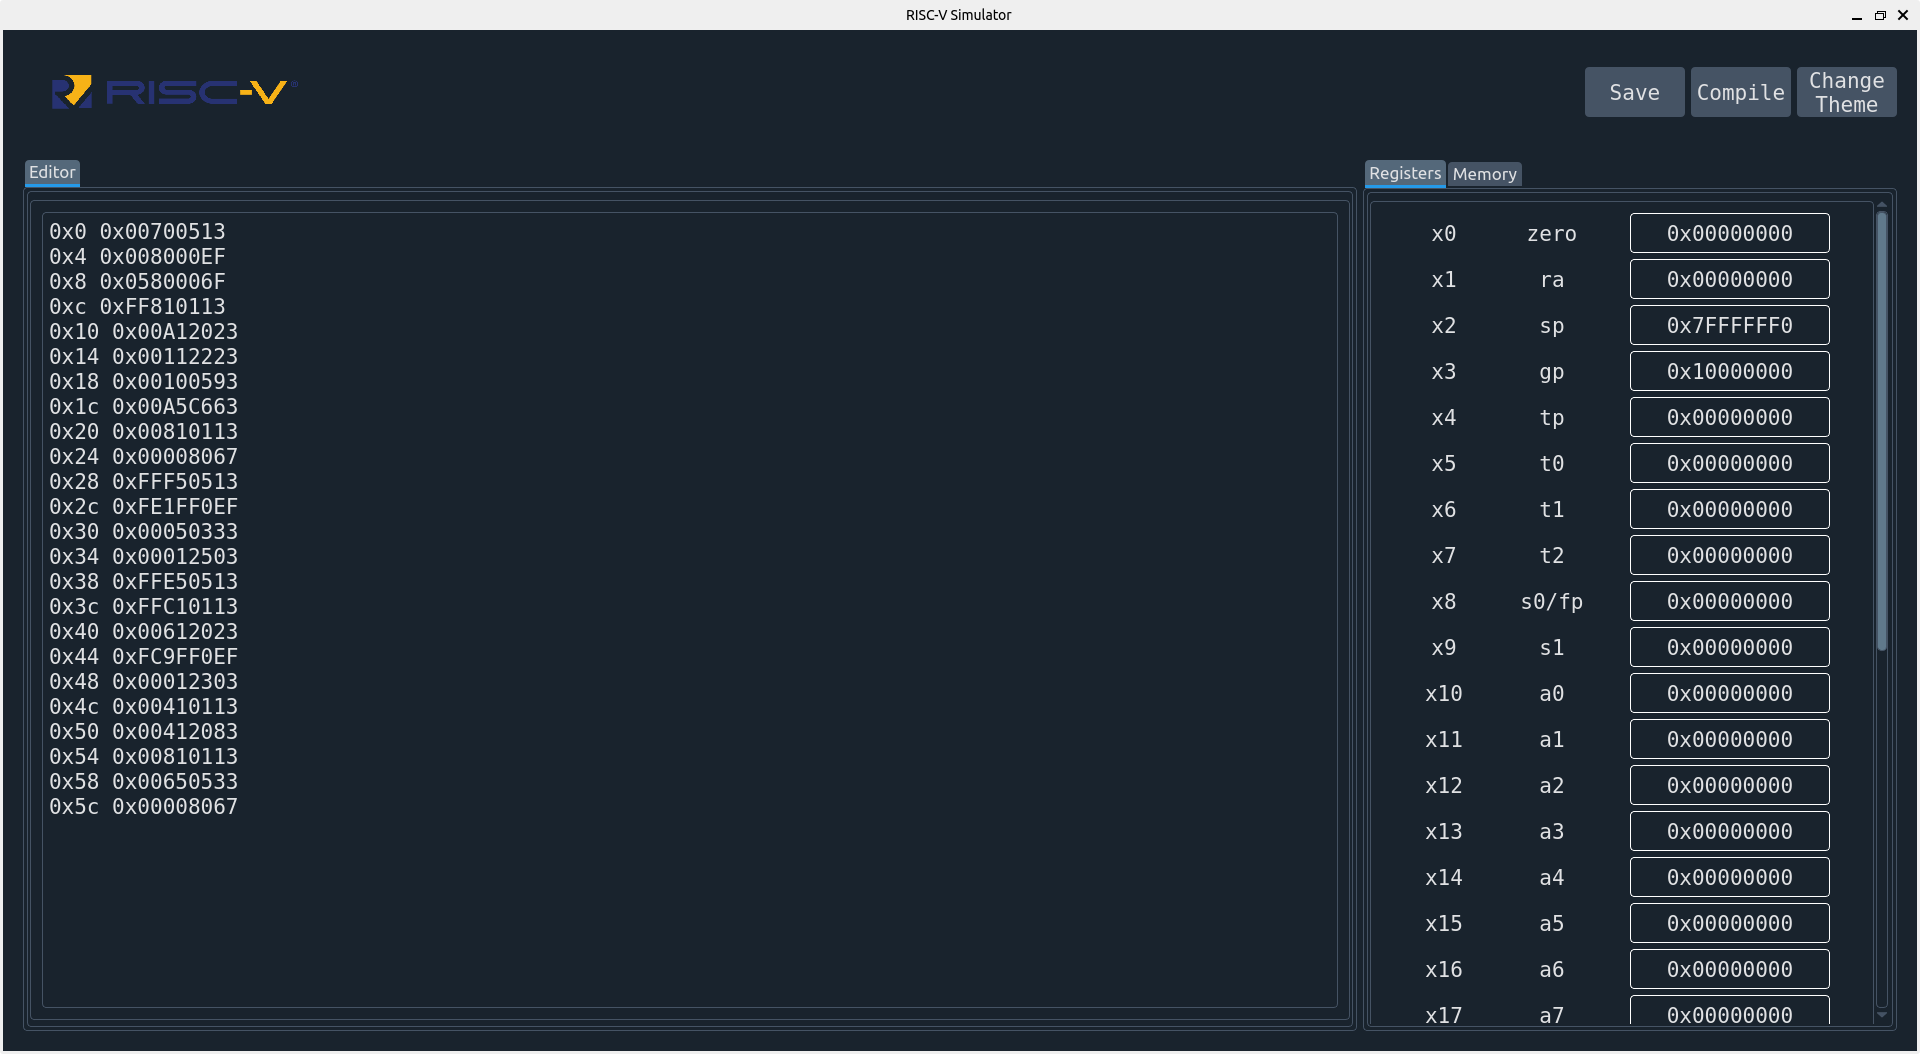
\includegraphics[width=1.0\textwidth]{pic2.png}
\end{centering}
\def\checkmark{\tikz\fill[scale=0.4](0,.35) -- (.25,0) -- (1,.7) -- (.25,.15) -- cycle;}
\LARGE
\\\\
We have made GUI in both light and dark theme. The theme can be changed using the button ``Change theme" on the top right.
We have shown memory and registers on the right part of the GUI while on the left part there is Code Editor.
First of all we will paste the code in the Editor on the left side and then save and compile the code by clicking the respective `save' and `compile' button. The code will get updated in main.mc file and then the code will be executed and a \checkmark\hspace{0.7mm} will appear. The memory and registers will be updated simultaneously.\\
We can jump in the memory using `Jump to' on the bottom right in memory section.\\
We can see all the registers in the register file by scrolling in the register file section.\\
Executing main.py always generates GUI window and you can code in Editor.
We can also execute non GUI code by writing python main.py 2

\newpage
\begin{centering}
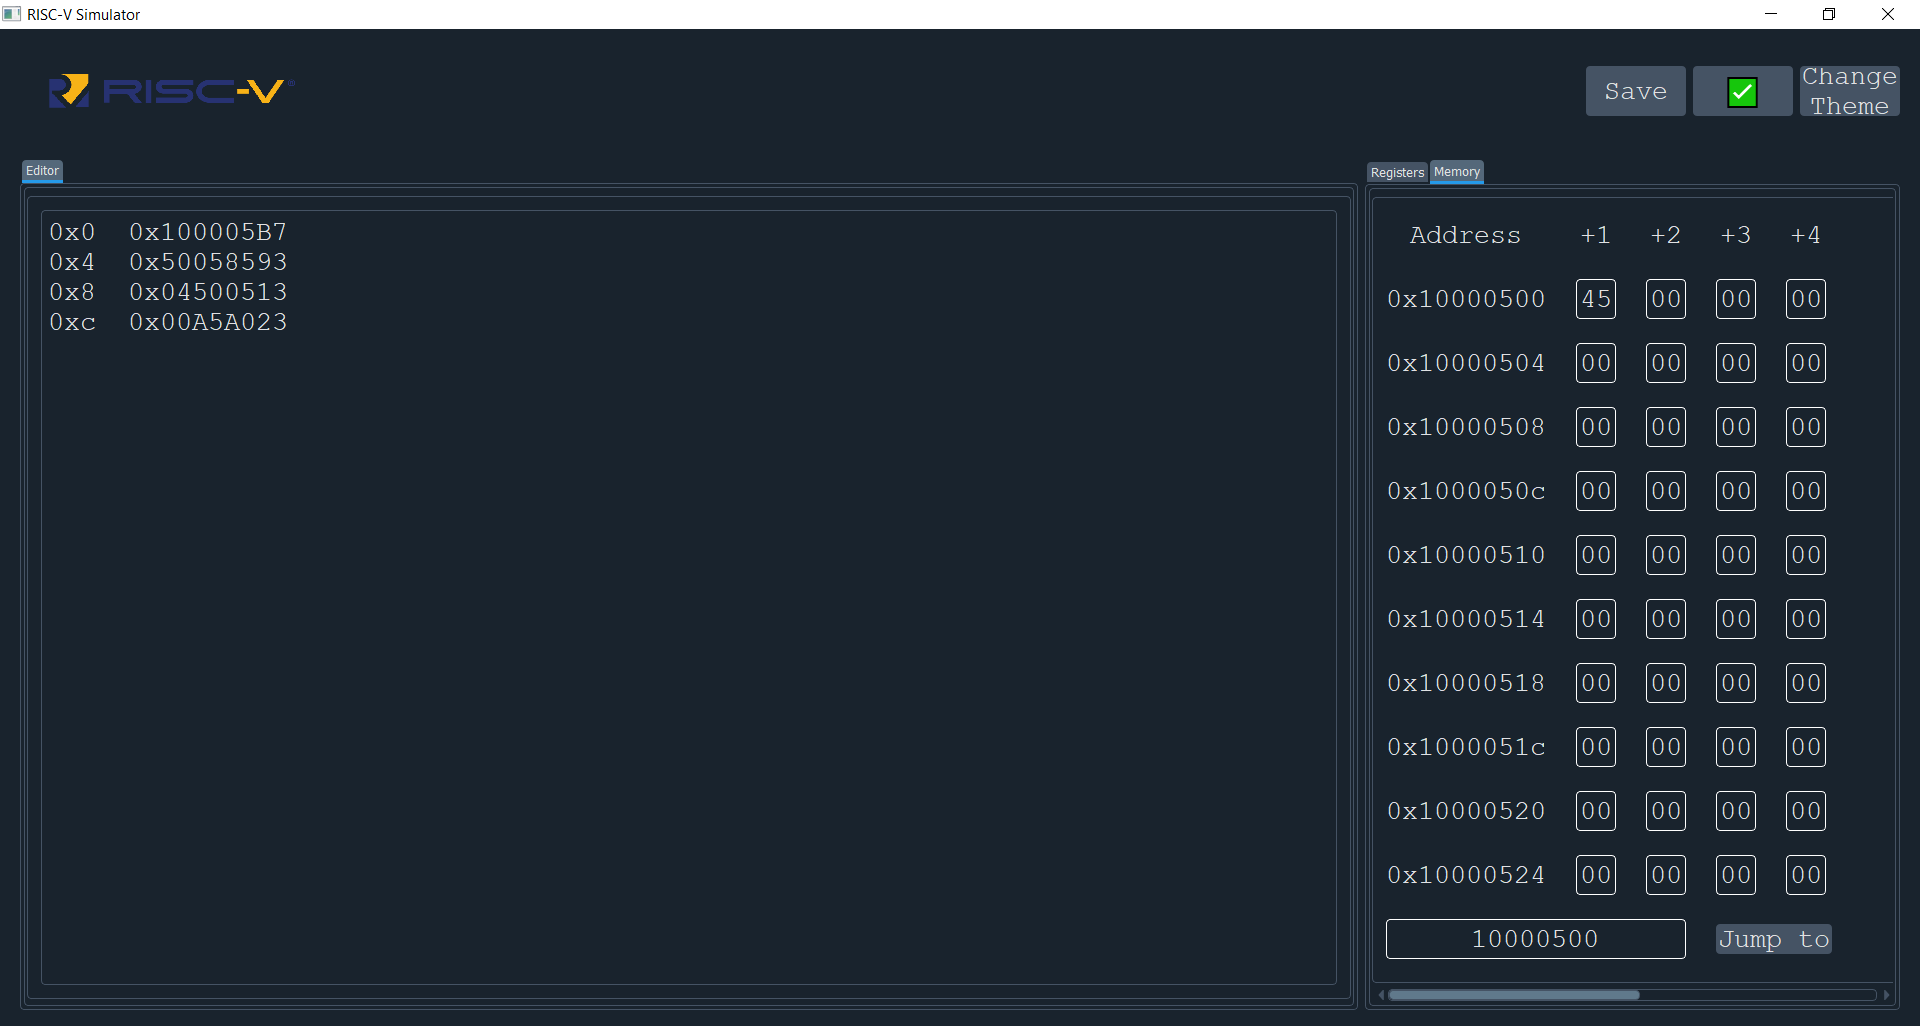
\includegraphics[width=1.0\textwidth]{pic3.png}
\end{centering}
\\\\
Here we can see the jump to register functionality, where we have stored a value in the register 0x10000500, and are jumping to it and seeing the value.
\newpage
\begin{centering}
\begin{Huge}
\textsf{Input/Output format details}\\
\end{Huge}
\vspace{0.6cm}
\end{centering}
\noindent
{\bf Input Format:}\\\\
0x0 0x00500513\\
0x4 0x008000EF\\
0x8 0x0440006F\\
\$\\
0x10000000 0x64\\

The section given before the `\$' sign is the text segment of the code and all the lines after it signify the data segment of the code.\\\\
Output is generated in the `generated' folder. `registers.txt' contains the register values, the `memory.txt' contains the memory part and the `outputLog.txt' contains the registers, memory and other details at each stage. \\\\
\textsl{\textbf{ An example output for OutputLog.txt is given as follows:}}\\
Fetch stage:\\
The value of PC is : 00000000\\
The instruction in IR is : 10000597\\
Decode stage:\\
code : {`neumonic': `auipc', `opcode': `0b0010111', `immediate':\\ `00010000000000000000000000000000', `rd': `01011', `format': `U', `id': 25}\\
rd is : 11\\
imm is : 10000000\\
Execute stage:\\
operand1 is 00000000 operand2 is: 10000000\\
RZ is : 10000000\\
Memory Access stage:\\
Register Update Stage:\\
RD: RY: 11 10000000\\
cycle is : 1\\
\end{document}
